%! Author = dboldog, tbubenik
%! Date = 03/05/2026

\documentclass[11pt, a4paper]{article}

\usepackage[utf8]{inputenc}
\usepackage[T1]{fontenc}
\usepackage{lmodern}
\usepackage[margin=2.5cm]{geometry}
\usepackage{graphicx}
\usepackage{hyperref}
\usepackage[protrusion=true, expansion=false]{microtype}
\usepackage{booktabs}
\usepackage{float}
\usepackage{xcolor}
\usepackage{listings}
\usepackage{array}

\hypersetup{
    colorlinks=true,
    linkcolor=black,
    citecolor=black,
    urlcolor=blue!70!black,
    hypertexnames=false
}

\lstset{
    basicstyle=\ttfamily\small,
    breaklines=true,
    frame=single,
    numbers=left,
    numberstyle=\tiny\color{gray},
    xleftmargin=2em,
    framexleftmargin=1.5em,
    columns=fullflexible
}

% Slovak language pack
\usepackage[slovak]{babel}

\newcommand{\LabelProtocol}{Protokol k zadaniu}
\newcommand{\LabelCourse}{Databázové technológie}
\newcommand{\LabelCode}{DBS}
\newcommand{\LabelUniversity}{Slovenská technická univerzita v~Bratislave}
\newcommand{\LabelFaculty}{Fakulta informatiky a~informačných technológií}
\newcommand{\LabelAssignment}{Zadanie}
\newcommand{\LabelStudent}{Študent}
\newcommand{\LabelTeacher}{Cvičiaci}
\newcommand{\LabelGroup}{Študijná skupina}
\newcommand{\LabelDate}{Dátum}
\newcommand{\LabelYear}{Akademický rok}
\newcommand{\LabelContents}{Obsah}
\graphicspath{{../assets/}}

\newcommand{\StudentName}{Dávid Boldog, Tomáš Bubeník}
\newcommand{\StudyGroup}{Štvrtok 11:00}
\newcommand{\TeacherName}{Ing. Matej Petrík}
\newcommand{\AssignmentNumber}{3}
\newcommand{\AssignmentTitle}{Implementácia fyzického modelu a procesov}
\newcommand{\ProjectTheme}{Reštauračný systém}
\newcommand{\AcademicYear}{2025/2026}

\begin{document}

\begin{titlepage}
    \centering

    \includegraphics[width=0.3\textwidth]{logo}

    \vspace{0.3cm}
    {\large \LabelUniversity}\\[2pt]
    {\large \LabelFaculty}

    \vspace{2.2cm}
    {\Huge\bfseries \LabelProtocol}

    \vspace{0.6cm}
    {\LARGE \LabelCode{} --- \LabelCourse}

    \vspace{0.4cm}
    {\Large \LabelAssignment{} \AssignmentNumber: \AssignmentTitle}

    \vspace{0.4cm}
    {\Large\bfseries \ProjectTheme}

    \vfill

    \begin{tabular}{r l}
        \textbf{\LabelStudent:} & \StudentName  \\[4pt]
        \textbf{\LabelGroup:}   & \StudyGroup   \\[4pt]
        \textbf{\LabelTeacher:} & \TeacherName  \\[4pt]
        \textbf{\LabelYear:}    & \AcademicYear \\[4pt]
        \textbf{\LabelDate:}    & \today        \\
    \end{tabular}

    \vspace{1.5cm}
\end{titlepage}

\renewcommand{\contentsname}{\LabelContents}
\tableofcontents
\clearpage

% Titulná stránka je kapitola 1 podľa zadania, preto číslovanie začína sekciou 2.
\setcounter{section}{1}

\section{Zmeny oproti Zadaniu 1}

Model ostal tematicky aj vzťahovo rovnaký ako v Zadaní 1: jadrom systému je spoločná tabuľka
\texttt{Objednavka}, ktorú špecializujú tabuľky \texttt{DineInObjednavka} a
\texttt{DeliveryObjednavka}. Pri implementácii fyzického modelu sme doplnili konkrétne
PostgreSQL dátové typy, ENUM hodnoty, referenčné akcie a indexy potrebné pre procesy v tomto
zadaní.

Najdôležitejšie spresnenia voči návrhu sú:
\begin{itemize}
    \item stavové atribúty sú implementované ako PostgreSQL ENUM typy,
    \item historická cena položky objednávky je uložená v \texttt{ObjednavkaPolozka.cena\_v\_case\_objednavky},
    \item prekrývanie rezervácií sa nevynucuje cez \texttt{CHECK}, pretože ide o medziriadkové pravidlo; procesy ho kontrolujú dotazom,
    \item vzťahy \texttt{Objednavka}--\texttt{Faktura} a \texttt{Objednavka}--\texttt{Recenzia} sú spresnené ako voliteľné 1:1; oproti pôvodnému diagramu sme opravili kardinalitu na strane faktúry a recenzie z \texttt{0..*} na \texttt{0..1},
    \item proces vytvorenia dine-in objednávky po úspešnom overení prepne rezerváciu do stavu \texttt{aktivna}.
\end{itemize}

\begin{figure}[H]
    \centering
    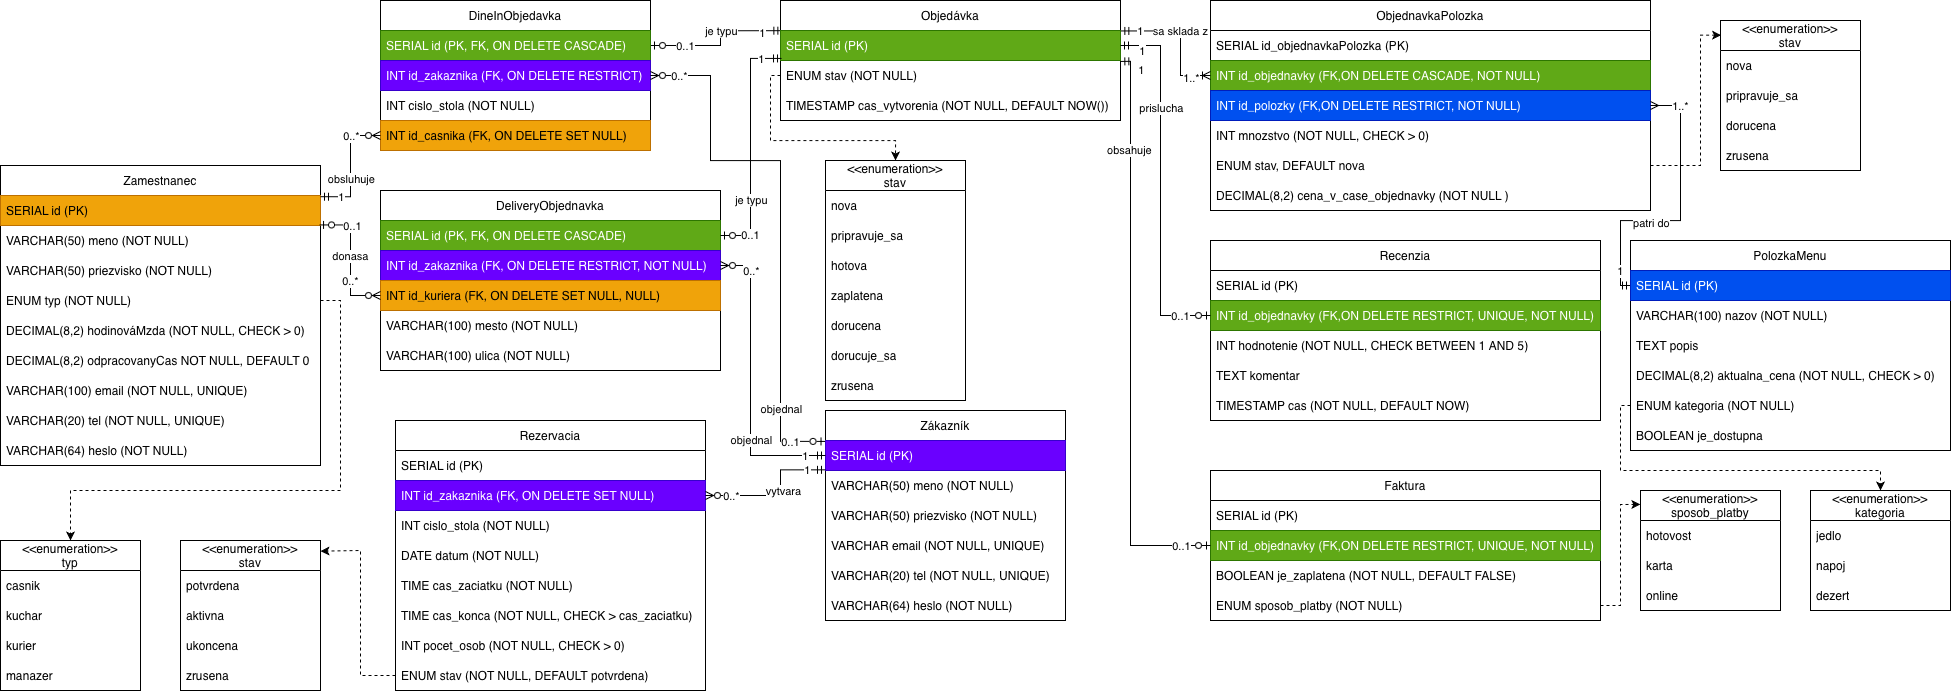
\includegraphics[width=\textwidth]{diagram}
    \caption{Aktuálny fyzický model databázy}
\end{figure}

\clearpage
\section{Fyzický model - implementácia}

Fyzický model je implementovaný v súbore \texttt{schema.sql}. Skript najprv odstráni existujúce
tabuľky a ENUM typy, následne vytvorí všetky typy, tabuľky, integritné obmedzenia a vlastné indexy.

\begin{table}[H]
\centering
\small
\begin{tabular}{p{4cm} p{10cm}}
\toprule
\textbf{Tabuľka} & \textbf{Účel} \\
\midrule
\texttt{Zamestnanec} & Evidencia čašníkov, kuchárov, kuriérov a manažérov. \\
\texttt{Zakaznik} & Registrovaní zákazníci pre rezervácie, dine-in a donášku. \\
\texttt{PolozkaMenu} & Aktuálna ponuka jedál, nápojov a dezertov. \\
\texttt{Objednavka} & Spoločná entita pre všetky objednávky. \\
\texttt{DineInObjednavka} & Špecializácia objednávky pri stole. \\
\texttt{DeliveryObjednavka} & Špecializácia donáškovej objednávky. \\
\texttt{ObjednavkaPolozka} & M:N vzťah objednávky a menu položiek so snímkou ceny. \\
\texttt{Rezervacia} & Rezervácia konkrétneho stola v časovom intervale. \\
\texttt{Faktura} & Platobný doklad k objednávke. \\
\texttt{Recenzia} & Jedno hodnotenie k jednej objednávke. \\
\bottomrule
\end{tabular}
\caption{Zoznam fyzických tabuliek}
\end{table}

\subsection*{Integritné obmedzenia}

Model používa primárne kľúče typu \texttt{SERIAL}, cudzie kľúče, \texttt{NOT NULL},
\texttt{UNIQUE}, \texttt{CHECK} a \texttt{DEFAULT}. Netriviálne pravidlá sú:
\begin{itemize}
    \item \texttt{email} a \texttt{tel} sú unikátne pri zákazníkoch aj zamestnancoch,
    \item ceny, mzdy, množstvá a počet osôb musia byť kladné,
    \item hodnotenie recenzie je obmedzené na interval 1 až 5,
    \item koniec rezervácie musí byť po začiatku rezervácie,
    \item \texttt{Faktura.id\_objednavky} a \texttt{Recenzia.id\_objednavky} sú unikátne, teda k objednávke existuje najviac jedna faktúra a najviac jedna recenzia.
\end{itemize}

\subsection*{Väzba na biznis pravidlá zo Zadania 1}

Fyzický model a seed dáta boli skontrolované voči pravidlám zo Zadania 1. Jednoznačnosť kontaktov
zákazníkov a zamestnancov vynucujú \texttt{UNIQUE} obmedzenia na \texttt{email} a \texttt{tel} a
generátor používa unikátne hodnoty. Kladné ceny, mzdy, množstvá a počet osôb sú chránené
\texttt{CHECK} obmedzeniami a seed ich generuje iba v povolených rozsahoch. Delivery objednávka má
povinné mesto a ulicu, takže ju nemožno vložiť bez doručovacej adresy.

Dostupnosť menu položiek je chránená v procese vytvorenia objednávky cez filter
\texttt{je\_dostupna = TRUE}; seed zároveň vyberá do objednávok iba dostupné položky. Historická cena
je uložená priamo v \texttt{ObjednavkaPolozka.cena\_v\_case\_objednavky}, takže zmeny aktuálnej ceny menu
neskreslia staré objednávky. Jedinečnosť faktúry a recenzie na objednávku vynucuje
\texttt{UNIQUE} na \texttt{id\_objednavky}; seed negeneruje duplicitné faktúry ani duplicitné recenzie.

Pravidlo neprekrývania rezervácií je medziriadkové. V schéme je preto priamo vynútený aspoň platný
časový interval rezervácie (\texttt{cas\_konca > cas\_zaciatku}) a operačný proces pracuje iba s jednou
potvrdenou rezerváciou pre konkrétny stôl, zákazníka, dátum a čas. Seed bol upravený tak, aby sa
potvrdené a aktívne rezervácie rovnakého stola časovo neprekrývali.

\subsection*{ON DELETE stratégie}

\begin{itemize}
    \item \texttt{ON DELETE CASCADE} je použité medzi \texttt{Objednavka} a jej detailmi, aby sa neosireli špecializačné a položkové záznamy.
    \item \texttt{ON DELETE RESTRICT} chráni historické objednávky pred zmazaním zákazníka alebo položky menu, na ktorú sa odkazujú.
    \item \texttt{ON DELETE SET NULL} sa používa pri voliteľných väzbách na zamestnanca alebo zákazníka, kde chceme zachovať historický záznam aj po odstránení osoby.
\end{itemize}

\clearpage
\section{Seed dáta}

Seed dáta sú generované skriptom \texttt{seed/seed.py} pomocou knižnice Faker so slovenskou lokalizáciou
\texttt{sk\_SK}. Generovanie je reprodukovateľné, pretože skript používa fixný seed
\texttt{SEED = 42}. Výstupom je súbor \texttt{seed/seed.sql}, ktorý vkladá dáta do všetkých hlavných
tabuliek a na konci nastaví hodnoty sekvencií cez \texttt{setval}. Reprodukcia seedu je popísaná v
\texttt{seed/README.md}.

\begin{table}[H]
\centering
\small
\begin{tabular}{lr}
\toprule
\textbf{Tabuľka} & \textbf{Počet záznamov} \\
\midrule
\texttt{Zamestnanec} & 25 \\
\texttt{Zakaznik} & 600 \\
\texttt{PolozkaMenu} & 50 \\
\texttt{Rezervacia} & 1 500 \\
\texttt{Objednavka} & 4 000 \\
\texttt{DineInObjednavka} & 2 338 \\
\texttt{DeliveryObjednavka} & 1 662 \\
\texttt{ObjednavkaPolozka} & 10 764 \\
\texttt{Faktura} & 3 621 \\
\texttt{Recenzia} & 1 177 \\
\midrule
\textbf{Spolu} & \textbf{25 737} \\
\bottomrule
\end{tabular}
\caption{Počty záznamov po seede}
\end{table}

Distribúcia dát je biznisovo motivovaná: objednávky sú rozdelené približne na 60 \% dine-in a
40 \% delivery, zákazníci sú vyberaní váženou náhodnosťou, takže časť zákazníkov objednáva často a
časť vôbec. Rezervácie sú rozložené medzi minulosť, aktuálny deň a budúcnosť, pričom budúce
rezervácie neobsahujú dokončené stavy.

Konzistencia je zabezpečená poradím generovania dát. Najprv vznikajú referenčné entity
(\texttt{Zakaznik}, \texttt{Zamestnanec}, \texttt{PolozkaMenu}), potom rezervácie, objednávky,
špecializácie objednávok, položky, faktúry a recenzie. Generátor vyberá iba existujúce cudzie kľúče
a rešpektuje roly zamestnancov pri čašníkoch a kuriéroch.

\clearpage
\section{Proces 1 - Vytvorenie dine-in objednávky}

\subsection*{Popis procesu}

Proces pokrýva príchod zákazníka s rezerváciou a vytvorenie objednávky pri stole. Vstupom sú
číslo stola, zákazník, dátum a čas príchodu, čašník a tri objednávané položky s množstvami.
Výstupom je detail vytvorenej objednávky alebo zoznam validačných chýb.

Proces overuje existenciu zákazníka, potvrdenú rezerváciu v danom časovom okne, rolu čašníka a
dostupnosť všetkých položiek menu. Ak všetky kontroly prejdú, v jednom SQL príkaze sa aktivuje
rezervácia a vložia sa záznamy do \texttt{Objednavka}, \texttt{DineInObjednavka} a
\texttt{ObjednavkaPolozka}.

\subsection*{Väzba na scenár zo Zadania 1}

Proces priamo nadväzuje na Scenár č. 1 - Rezervácia stola a príchod do reštaurácie a na začiatok
Scenára č. 2 - Objednanie jedla, platba a recenzia. Zo Scenára č. 1 preberá overenie rezervácie pri
príchode zákazníka a jej prepnutie do stavu \texttt{aktivna}; zo Scenára č. 2 preberá vytvorenie
dine-in objednávky, kontrolu dostupných položiek menu a uloženie snímky ceny.

\subsection*{SQL implementácia}

Implementácia je v súbore \texttt{queries.sql}. Parametre a vstupné položky sa na začiatku uložia do
krátkych dočasných tabuliek, aby sa neopakovali vo všetkých dotazoch. Samotná validácia a zápisy
používajú \texttt{UPDATE}, \texttt{INSERT ... SELECT} a vnorené subqueries. Nepoužíva PL/pgSQL blok
\texttt{DO}, vlastné uložené funkcie, procedúry, triggery ani kurzory.
Nasledujúci výpis je skrátená kostra; úplná spustiteľná verzia je v súbore \texttt{queries.sql}.

\begin{lstlisting}
BEGIN;

CREATE TEMP TABLE tmp_p1_params ON COMMIT DROP AS
SELECT vstupne_parametre;

CREATE TEMP TABLE tmp_p1_items ON COMMIT DROP AS
SELECT polozka_id, mnozstvo
FROM vstupne_polozky;

CREATE TEMP TABLE tmp_p1_errors ON COMMIT DROP AS
SELECT sprava
FROM validacne_kontroly
WHERE pravidlo_neplati;

CREATE TEMP TABLE tmp_p1_order ON COMMIT DROP AS
SELECT nextval('objednavka_id_seq')::INT AS id_objednavky
WHERE NOT EXISTS (SELECT 1 FROM tmp_p1_errors);

-- nasleduju INSERTy do Objednavka, DineInObjednavka a ObjednavkaPolozka
-- a UPDATE potvrdenej rezervacie na stav aktivna

SELECT vysledok, sprava
FROM vystup_procesu;

COMMIT;
\end{lstlisting}

\subsection*{Ukážka spustenia}

Testovacie parametre v \texttt{queries.sql}:
\begin{itemize}
    \item stôl: 8,
    \item zákazník: \texttt{id = 320},
    \item čas príchodu: \texttt{2026-05-03 13:15},
    \item čašník: \texttt{id = 13},
    \item položky: \texttt{12 x 1}, \texttt{17 x 2}, \texttt{24 x 2}.
\end{itemize}

\begin{table}[H]
\centering
\small
\begin{tabular}{llrr}
\toprule
\textbf{Položka} & \textbf{Stav} & \textbf{Množstvo} & \textbf{Subtotal} \\
\midrule
Pizza Margherita & nova & 1 & 13.30 \\
Kurací burger & nova & 2 & 31.82 \\
Cappuccino & nova & 2 & 7.64 \\
\midrule
\textbf{Spolu} & & & \textbf{52.76} \\
\bottomrule
\end{tabular}
\caption{Očakávaný výstup procesu 1 nad seed dátami}
\end{table}

\subsection*{Zdôvodnenie korektnosti}

Objednávka sa vloží iba vtedy, keď dočasná tabuľka \texttt{tmp\_p1\_errors} ostane prázdna.
Všetky zápisy sú v jednej transakcii, takže nevznikne situácia, že sa vytvorí iba časť objednávky.
Snímka ceny sa berie z aktuálnej ceny v \texttt{PolozkaMenu} v momente vytvorenia objednávky.

\subsection*{Indexy podporujúce proces}

\begin{itemize}
    \item \texttt{idx\_rezervacia\_stol\_datum} podporuje hľadanie rezervácie podľa stola, dátumu a stavu.
    \item \texttt{idx\_polozka\_dostupna} podporuje filtrovanie dostupných položiek menu.
    \item \texttt{idx\_objednavkapolozka\_objednavka} zrýchľuje načítanie položiek vytvorenej objednávky.
\end{itemize}

\clearpage
\section{Proces 2 - Výkonnostný report čašníkov}

\subsection*{Popis procesu}

Manažér chce za zvolený rok vidieť výkon jednotlivých čašníkov. Report pracuje iba so zaplatenými
dine-in objednávkami, teda so záznamami, ku ktorým existuje faktúra s
\texttt{je\_zaplatena = TRUE}. Výstup obsahuje počet objednávok, celkovú tržbu, priemernú hodnotu
objednávky, priemerné hodnotenie, poradie podľa tržby, percentuálny podiel a kumulatívnu tržbu.

\subsection*{Väzba na scenár zo Zadania 1}

Proces využíva dáta, ktoré vznikajú v Scenári č. 2 - Objednanie jedla, platba a recenzia: dine-in
objednávky, položky objednávky, faktúry a recenzie. Zároveň nadväzuje na manažérsku rolu zo
špecifikácie Zadania 1, kde manažér generuje prevádzkové reporty a potrebuje prehľad o výkone
čašníkov.

\subsection*{SQL implementácia}

Proces používa pohľad \texttt{v\_dine\_in\_trzby}, vnorené subqueries, agregácie a window funkcie.
Rok sa filtruje cez rozsah dátumov, nie cez \texttt{EXTRACT(YEAR ...)}, aby databáza vedela
efektívnejšie použiť index na \texttt{Objednavka.cas\_vytvorenia}.

\begin{lstlisting}[language=SQL]
CREATE OR REPLACE VIEW v_dine_in_trzby AS
SELECT o.id, o.cas_vytvorenia, d.id_casnika,
       SUM(op.mnozstvo * op.cena_v_case_objednavky) AS trzba_objednavky
FROM Objednavka o
JOIN Faktura f ON f.id_objednavky = o.id AND f.je_zaplatena = TRUE
JOIN DineInObjednavka d ON d.id = o.id
JOIN ObjednavkaPolozka op ON op.id_objednavky = o.id
WHERE o.stav <> 'zrusena'
GROUP BY o.id, o.cas_vytvorenia, d.id_casnika;

SELECT w.id_casnika, z.meno, z.priezvisko,
       w.pocet_objednavok, w.celkova_trzba,
       w.avg_hodnotenie, w.poradie
FROM (
    SELECT s.*, h.avg_hodnotenie,
           RANK() OVER (ORDER BY s.celkova_trzba DESC) AS poradie
    FROM (
        SELECT id_casnika, COUNT(*) AS pocet_objednavok,
               SUM(trzba_objednavky) AS celkova_trzba
        FROM v_dine_in_trzby
        WHERE cas_vytvorenia >= '2026-01-01'
          AND cas_vytvorenia <  '2027-01-01'
        GROUP BY id_casnika
    ) s
    LEFT JOIN (
        SELECT d.id_casnika, AVG(r.hodnotenie) AS avg_hodnotenie
        FROM Recenzia r
        JOIN Objednavka o ON o.id = r.id_objednavky
        JOIN DineInObjednavka d ON d.id = o.id
        GROUP BY d.id_casnika
    ) h ON h.id_casnika = s.id_casnika
) w
JOIN Zamestnanec z ON z.id = w.id_casnika;
\end{lstlisting}

\subsection*{Ukážka výstupu}

\begin{table}[H]
\centering
\small
\begin{tabular}{rlrrrr}
\toprule
\textbf{Poradie} & \textbf{Čašník} & \textbf{Obj.} & \textbf{Tržba} & \textbf{Priemer} & \textbf{Hodn.} \\
\midrule
1 & Kristián Kučerová & 47 & 3001.85 & 63.87 & 4.13 \\
2 & Ľubomíra Miklošová & 46 & 2797.38 & 60.81 & 4.00 \\
3 & Metod Huba & 38 & 2528.98 & 66.55 & 3.75 \\
4 & Leonard Macháčeková & 34 & 2460.25 & 72.36 & 3.75 \\
5 & Irena Janečková & 35 & 2435.39 & 69.58 & 3.93 \\
\bottomrule
\end{tabular}
\caption{Prvých päť riadkov reportu pre rok 2026}
\end{table}

\subsection*{Zdôvodnenie korektnosti}

Tržba vzniká ako súčet \texttt{mnozstvo * cena\_v\_case\_objednavky}, teda používa historickú cenu
uloženú v objednávke, nie aktuálnu cenu menu. Zrušené objednávky a zrušené položky sa do reportu
nezapočítavajú. Join na \texttt{Faktura} zabezpečí, že report reprezentuje reálne zaplatené tržby.

\subsection*{Indexy podporujúce proces}

\begin{itemize}
    \item \texttt{idx\_objednavka\_cas\_vytvorenia} podporuje rozsahový filter zvoleného roka.
    \item \texttt{idx\_faktura\_zaplatena} podporuje výber zaplatených faktúr a join na objednávku.
    \item \texttt{idx\_objednavkapolozka\_objednavka} podporuje agregáciu položiek podľa objednávky.
\end{itemize}

\clearpage
\section{Výkonnosť a indexy}

PostgreSQL automaticky vytvára indexy pre \texttt{PRIMARY KEY} a \texttt{UNIQUE} obmedzenia.
Tieto indexy sa do požadovaného minima nepočítajú. V schéme preto vytvárame päť vlastných
indexov, ktoré priamo podporujú dva implementované procesy.

\subsection*{\texttt{idx\_rezervacia\_stol\_datum}}

\begin{lstlisting}[language=SQL]
CREATE INDEX idx_rezervacia_stol_datum
    ON Rezervacia (cislo_stola, datum, stav);
\end{lstlisting}

Index podporuje proces 1, konkrétne validáciu rezervácie pred vytvorením dine-in objednávky.
Dopyt filtruje tabuľku \texttt{Rezervacia} podľa \texttt{cislo\_stola}, \texttt{datum} a
\texttt{stav}. Bez indexu musí databáza prejsť všetky rezervácie sekvenčným skenom a až potom
odfiltrovať konkrétny stôl, dátum a stav. Index má odstrániť práve tento sekvenčný sken nad
tabuľkou \texttt{Rezervacia}; zvyšné podmienky na zákazníka a časový interval sa potom aplikujú
iba na malú množinu kandidátov.

\subsection*{\texttt{idx\_polozka\_dostupna}}

\begin{lstlisting}[language=SQL]
CREATE INDEX idx_polozka_dostupna
    ON PolozkaMenu (je_dostupna);
\end{lstlisting}

Index podporuje proces 1 pri validácii, že objednávané položky menu existujú a sú dostupné.
Dopyt používa podmienku \texttt{je\_dostupna = TRUE}. Cieľom indexu je obmedziť skenovanie
nedostupných položiek pri zostavovaní dostupného menu alebo pri validácii vstupu objednávky.
Keďže tabuľka menu je v našom seede malá, optimalizátor môže aj tak zvoliť sekvenčný sken; index
je však opodstatnený pre prípad väčšieho menu alebo častého filtrovania dostupných položiek.

\subsection*{\texttt{idx\_objednavkapolozka\_objednavka}}

\begin{lstlisting}[language=SQL]
CREATE INDEX idx_objednavkapolozka_objednavka
    ON ObjednavkaPolozka (id_objednavky);
\end{lstlisting}

Index podporuje oba procesy. V procese 1 sa používa pri načítaní detailu novo vytvorenej
objednávky a v procese 2 pri agregácii tržby objednávky. Dopyty často hľadajú všetky riadky
\texttt{ObjednavkaPolozka} pre jedno konkrétne \texttt{id\_objednavky}. PostgreSQL nevytvára index
automaticky na stĺpci cudzieho kľúča, preto je tento index vlastný. Má obmedziť sekvenčný sken
celej tabuľky položiek objednávok a nahradiť ho indexovým vyhľadaním položiek konkrétnej
objednávky.

\subsection*{\texttt{idx\_objednavka\_cas\_vytvorenia}}

\begin{lstlisting}[language=SQL]
CREATE INDEX idx_objednavka_cas_vytvorenia
    ON Objednavka (cas_vytvorenia);
\end{lstlisting}

Index podporuje proces 2, kde manažérsky report filtruje objednávky za zvolený rok. Dopyt je
zámerne zapísaný ako rozsah:

\begin{lstlisting}[language=SQL]
WHERE o.cas_vytvorenia >= y.rok_od
  AND o.cas_vytvorenia <  y.rok_do
\end{lstlisting}

Takýto zápis je vhodný pre B-tree index nad \texttt{cas\_vytvorenia}. Index má obmedziť
sekvenčné skenovanie všetkých objednávok pri ročných reportoch. Keby bol filter zapísaný ako
\texttt{EXTRACT(YEAR FROM cas\_vytvorenia)}, databáza by musela vypočítať výraz pre každý riadok
a tento index by sa používal horšie alebo vôbec.

\subsection*{\texttt{idx\_faktura\_zaplatena}}

\begin{lstlisting}[language=SQL]
CREATE INDEX idx_faktura_zaplatena
    ON Faktura (je_zaplatena, id_objednavky);
\end{lstlisting}

Index podporuje proces 2. Report má počítať iba reálne tržby, preto pohľad
\texttt{v\_dine\_in\_trzby} joinuje tabuľku \texttt{Faktura} a filtruje
\texttt{je\_zaplatena = TRUE}. Prvý stĺpec indexu podporuje filter zaplatených faktúr, druhý stĺpec
podporuje následný join na \texttt{Objednavka.id}. Index má obmedziť sekvenčný sken tabuľky
\texttt{Faktura} pri hľadaní zaplatených objednávok.

\subsection*{EXPLAIN porovnanie}

Porovnanie sme spravili pre proces 1, konkrétne pre validáciu rezervácie. Test bol spustený nad
naplnenou databázou so seed dátami. Najprv sme index \texttt{idx\_rezervacia\_stol\_datum}
odstránili a spustili plán:

\begin{lstlisting}[language=SQL]
DROP INDEX IF EXISTS idx_rezervacia_stol_datum;

EXPLAIN (ANALYZE, BUFFERS)
SELECT r.id, r.id_zakaznika, r.cislo_stola, r.datum,
       r.cas_zaciatku, r.cas_konca, r.stav
FROM Rezervacia r
WHERE r.cislo_stola = 8
  AND r.id_zakaznika = 320
  AND r.datum = DATE '2026-05-03'
  AND TIME '13:15' BETWEEN r.cas_zaciatku AND r.cas_konca
  AND r.stav = 'potvrdena'
ORDER BY r.id
LIMIT 1;
\end{lstlisting}

Výrez plánu bez indexu:

\begin{lstlisting}
Limit  (actual time=0.164..0.164 rows=1 loops=1)
  Buffers: shared hit=16
  ->  Sort
        Sort Key: id
        ->  Seq Scan on rezervacia r
              Rows Removed by Filter: 1499
              Buffers: shared hit=13
Planning Time: 0.531 ms
Execution Time: 0.189 ms
\end{lstlisting}

Bez indexu databáza použila \texttt{Seq Scan on rezervacia}. To znamená, že prešla všetkých
1 500 rezervácií a 1 499 riadkov zahodila filtrom.

Následne sme index vytvorili znova a spustili ten istý dopyt:

\begin{lstlisting}[language=SQL]
CREATE INDEX idx_rezervacia_stol_datum
    ON Rezervacia (cislo_stola, datum, stav);

ANALYZE Rezervacia;

EXPLAIN (ANALYZE, BUFFERS)
SELECT r.id, r.id_zakaznika, r.cislo_stola, r.datum,
       r.cas_zaciatku, r.cas_konca, r.stav
FROM Rezervacia r
WHERE r.cislo_stola = 8
  AND r.id_zakaznika = 320
  AND r.datum = DATE '2026-05-03'
  AND TIME '13:15' BETWEEN r.cas_zaciatku AND r.cas_konca
  AND r.stav = 'potvrdena'
ORDER BY r.id
LIMIT 1;
\end{lstlisting}

Výrez plánu s indexom:

\begin{lstlisting}
Limit  (actual time=0.037..0.037 rows=1 loops=1)
  Buffers: shared hit=1 read=2
  ->  Sort
        Sort Key: id
        ->  Index Scan using idx_rezervacia_stol_datum on rezervacia r
              Index Cond: ((cislo_stola = 8)
                           AND (datum = '2026-05-03'::date)
                           AND (stav = 'potvrdena'::stav_rezervacie))
              Filter: (id_zakaznika = 320
                       AND '13:15'::time BETWEEN cas_zaciatku AND cas_konca)
Planning Time: 0.264 ms
Execution Time: 0.059 ms
\end{lstlisting}

Po vytvorení indexu sa plán zmenil zo sekvenčného skenu na \texttt{Index Scan}. Databáza už
nehľadala rezerváciu v celej tabuľke, ale použila indexovú podmienku nad stĺpcami
\texttt{cislo\_stola}, \texttt{datum} a \texttt{stav}. Aj na relatívne malom seede klesol čas
vykonania z približne \texttt{0.189 ms} na \texttt{0.059 ms}. Zostalo iba malé triedenie podľa
\texttt{id}, pretože \texttt{id} nie je súčasťou indexu; triedi sa však už len veľmi malá množina
kandidátnych riadkov.

\clearpage
\section{Zhodnotenie}

Najnáročnejšou časťou bolo zosúladiť fyzický model s procesmi tak, aby procesy neboli iba
jednoduché SELECT dotazy, ale pokrývali reálnu prevádzkovú logiku. Pri procese 1 bolo dôležité
vytvoriť objednávku čisto v SQL bez PL/pgSQL, ale zároveň zachovať validačné kroky a atomickosť
zápisu.

Pri implementácii sa ukázalo, že niektoré biznis pravidlá nie je vhodné riešiť obyčajným
\texttt{CHECK} obmedzením. Typickým príkladom je prekrývanie rezervácií, ktoré vyžaduje kontrolu
voči iným riadkom. Toto pravidlo preto riešime validačným dotazom v procese.

Indexy sme nenavrhovali plošne na všetky stĺpce. Zamerali sme sa na časti dopytov, ktoré sa opakujú
v procesoch: hľadanie rezervácie podľa stola a dátumu, načítanie položiek objednávky, filter
zaplatených faktúr a rozsahový filter objednávok podľa dátumu.

AI nástroje sme použili ako pomoc pri kontrole konzistentnosti textu, formulácii reportu a
prepisovaní SQL procesu do čistej deklaratívnej podoby. Výsledné SQL a model sme skontrolovali
voči zadaniu a upravili podľa reálnych tabuliek v projekte.

\end{document}
